\documentclass[aspectratio=169,svgnames]{beamer}

\usepackage{lmodern}
\usepackage[T1]{fontenc}
\usepackage[ngerman]{babel}
\usepackage{selinput}
\SelectInputMappings{%
   adieresis={ä},
   germandbls={ß}
   }
\usepackage{csquotes}

\usepackage{hyperref}

\usepackage{siunitx}
\DeclareSIUnit\inch{in}
\DeclareSIUnit\in{in}

\usetheme{Rochester}  %% Themenwahl

\setbeamercovered{transparent}
%\setbeamertemplate{footline}[frame number]
% \usecolortheme{spruce}        % grün
% \usecolortheme{beetle}
\usecolortheme{cormorant}
% \usecolortheme[named=MSUgreen]{structure}
\newcommand{\hshblogo}{\includegraphics[width=1.3cm]{space-logo}}
\newcommand{\divider}[1]{\begin{frame} %
\begin{alertblock}{} %
\centering\usebeamerfont{section title}#1 %
\end{alertblock} %
\end{frame}}

\title{Ein mobiler CO2 Sensor}
\author{Syralist}
\date{17.06.2025}
\logo{
\includegraphics[width=1.1cm]{Syralist_Kalligraphie_Logo_rund}}
 
\begin{document}
\maketitle
% \frame{\tableofcontents}

\begin{frame}%[<+->] %%Eine Folie
    \frametitle{Ich habe einen mobilen CO2 Sensor gebaut} %%Folientitel
    \centering
    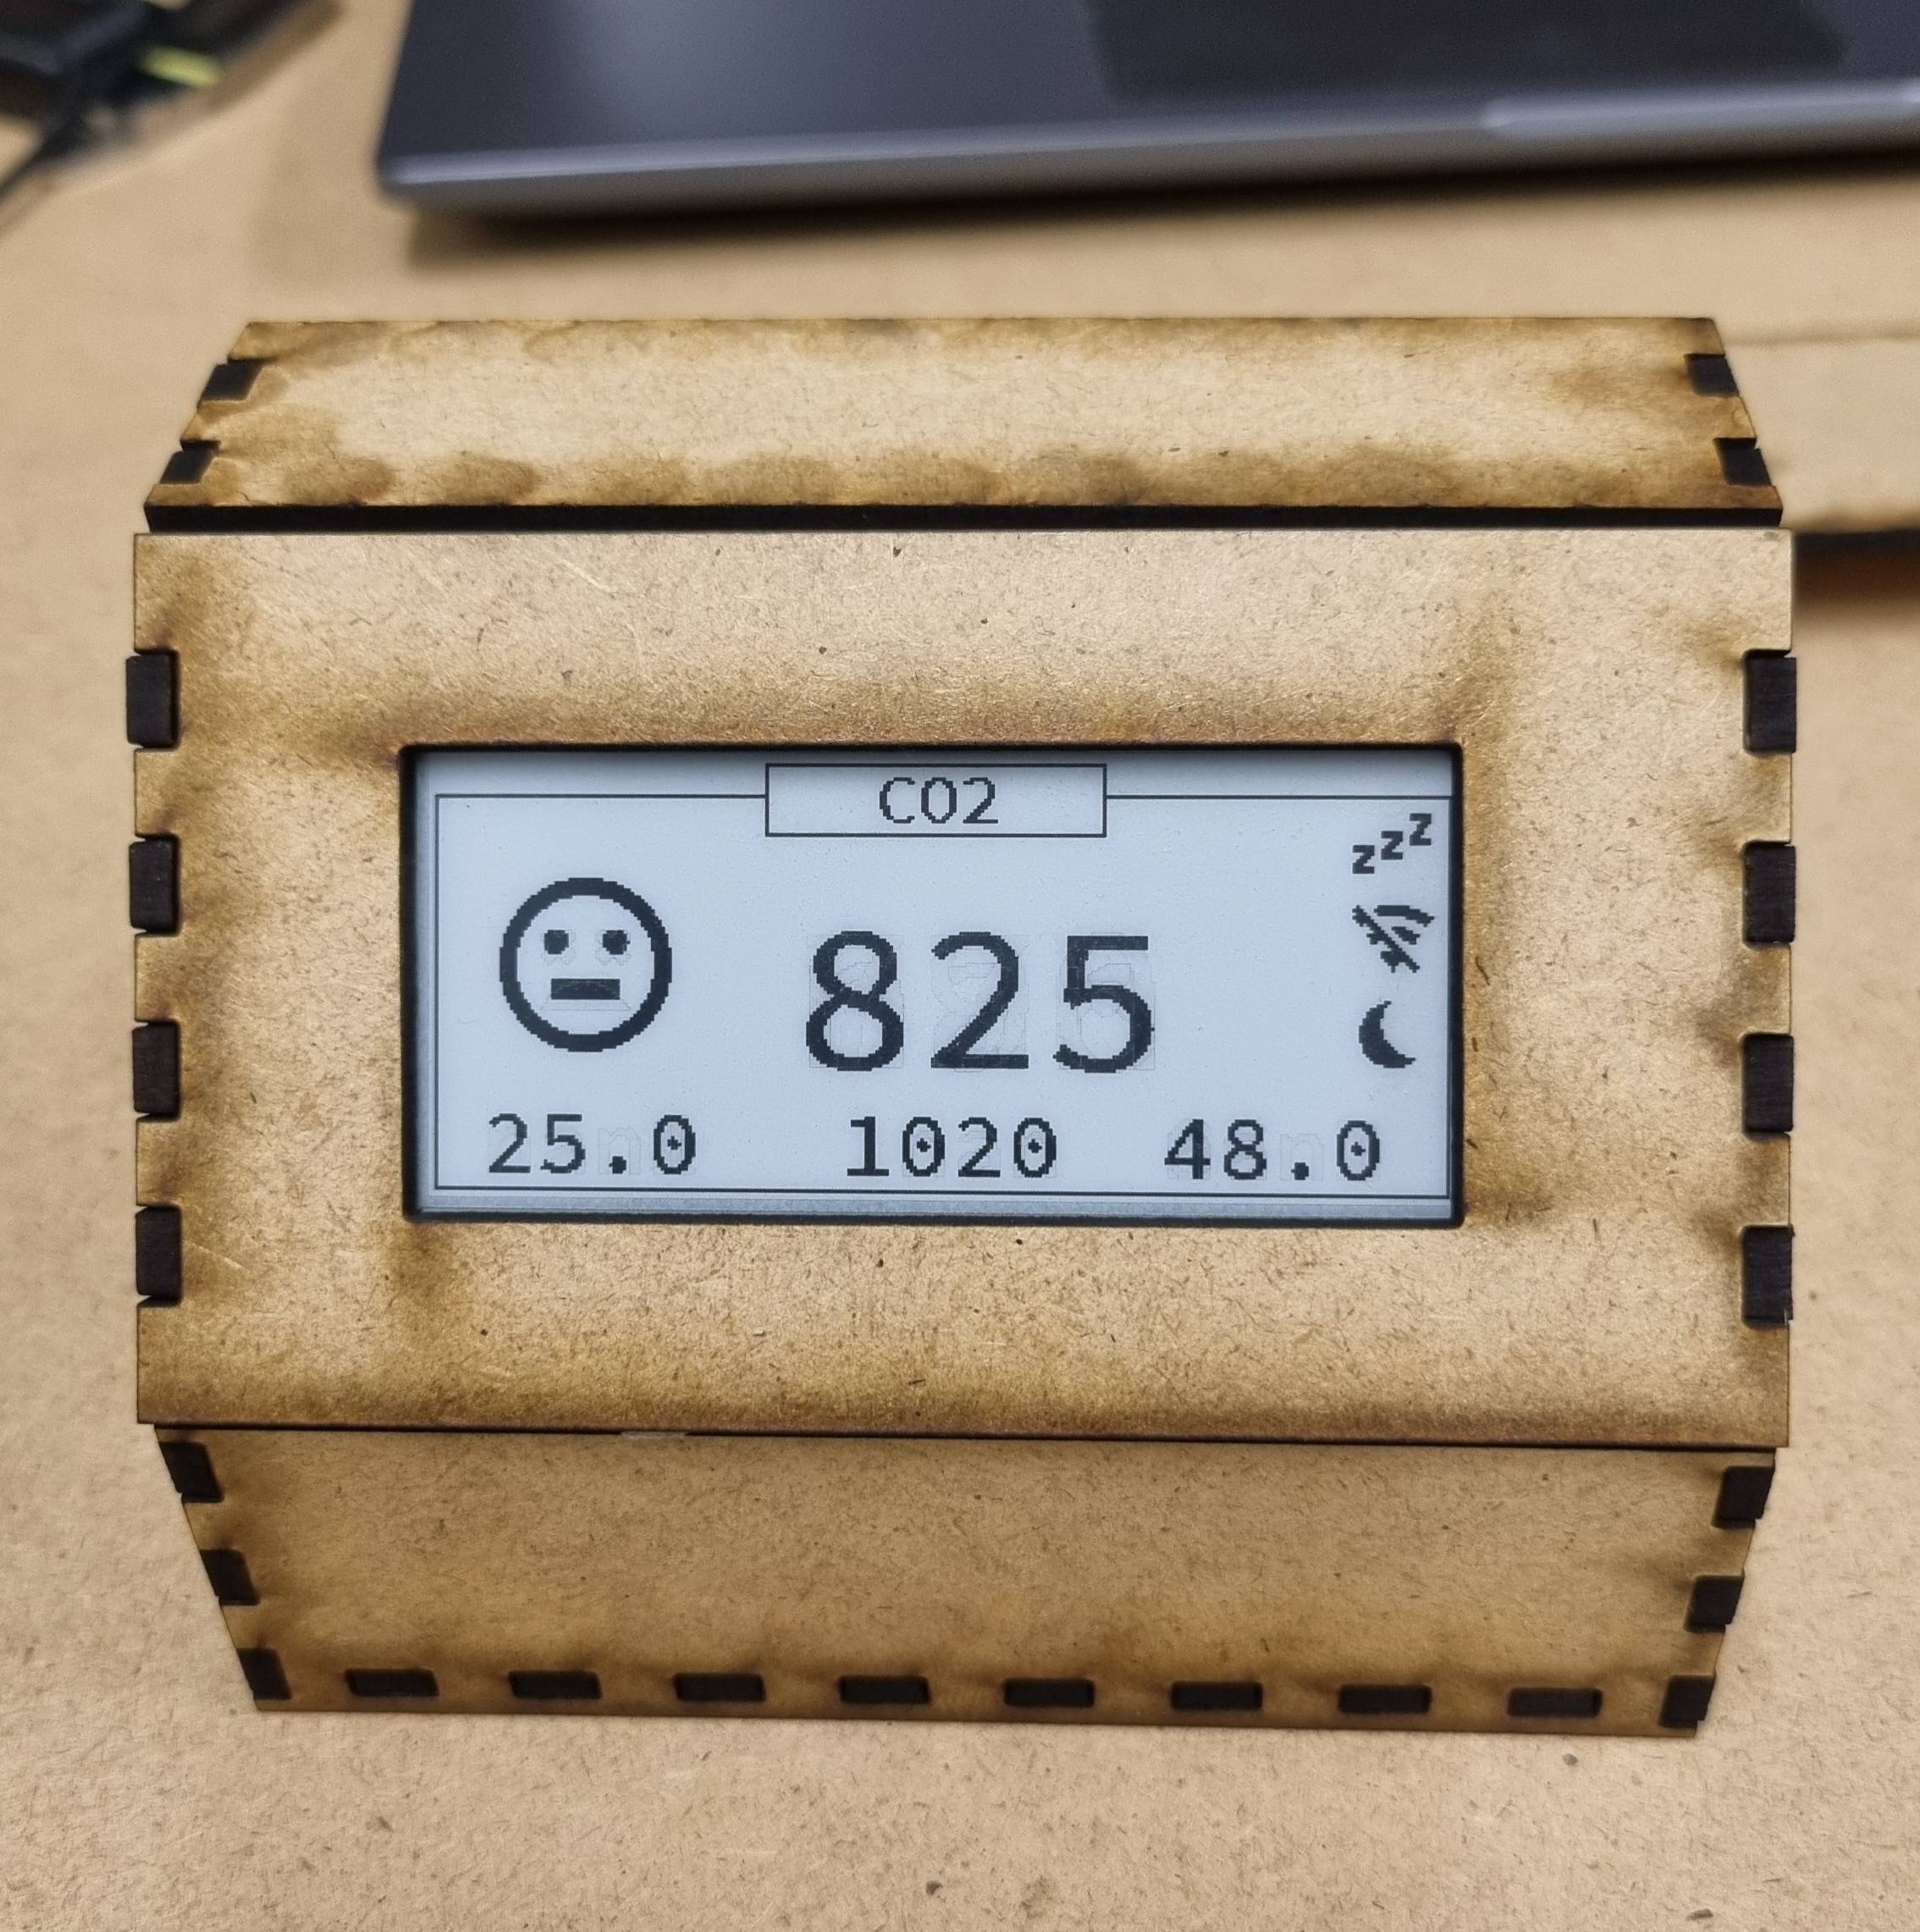
\includegraphics[height=0.9\textheight]{sensor-fertig-01.jpg}
\end{frame}

% \section{Motivation}
% \divider{\insertsection}
\begin{frame}%[<+->] %%Eine Folie
    \frametitle{Warum hab ich das gemacht?} %%Folientitel
    \begin{itemize}[<+->]
        \item Covid is not over
        \item Aranet ist teuer
        \item Das Display lag seit Jahren ungenutzt in einer Box
        \item Ich wollte sehen, ob ich das kann
    \end{itemize}
\end{frame}

\begin{frame}%[<+->] %%Eine Folie
    \frametitle{Die Bauteile} %%Folientitel
    \centering
    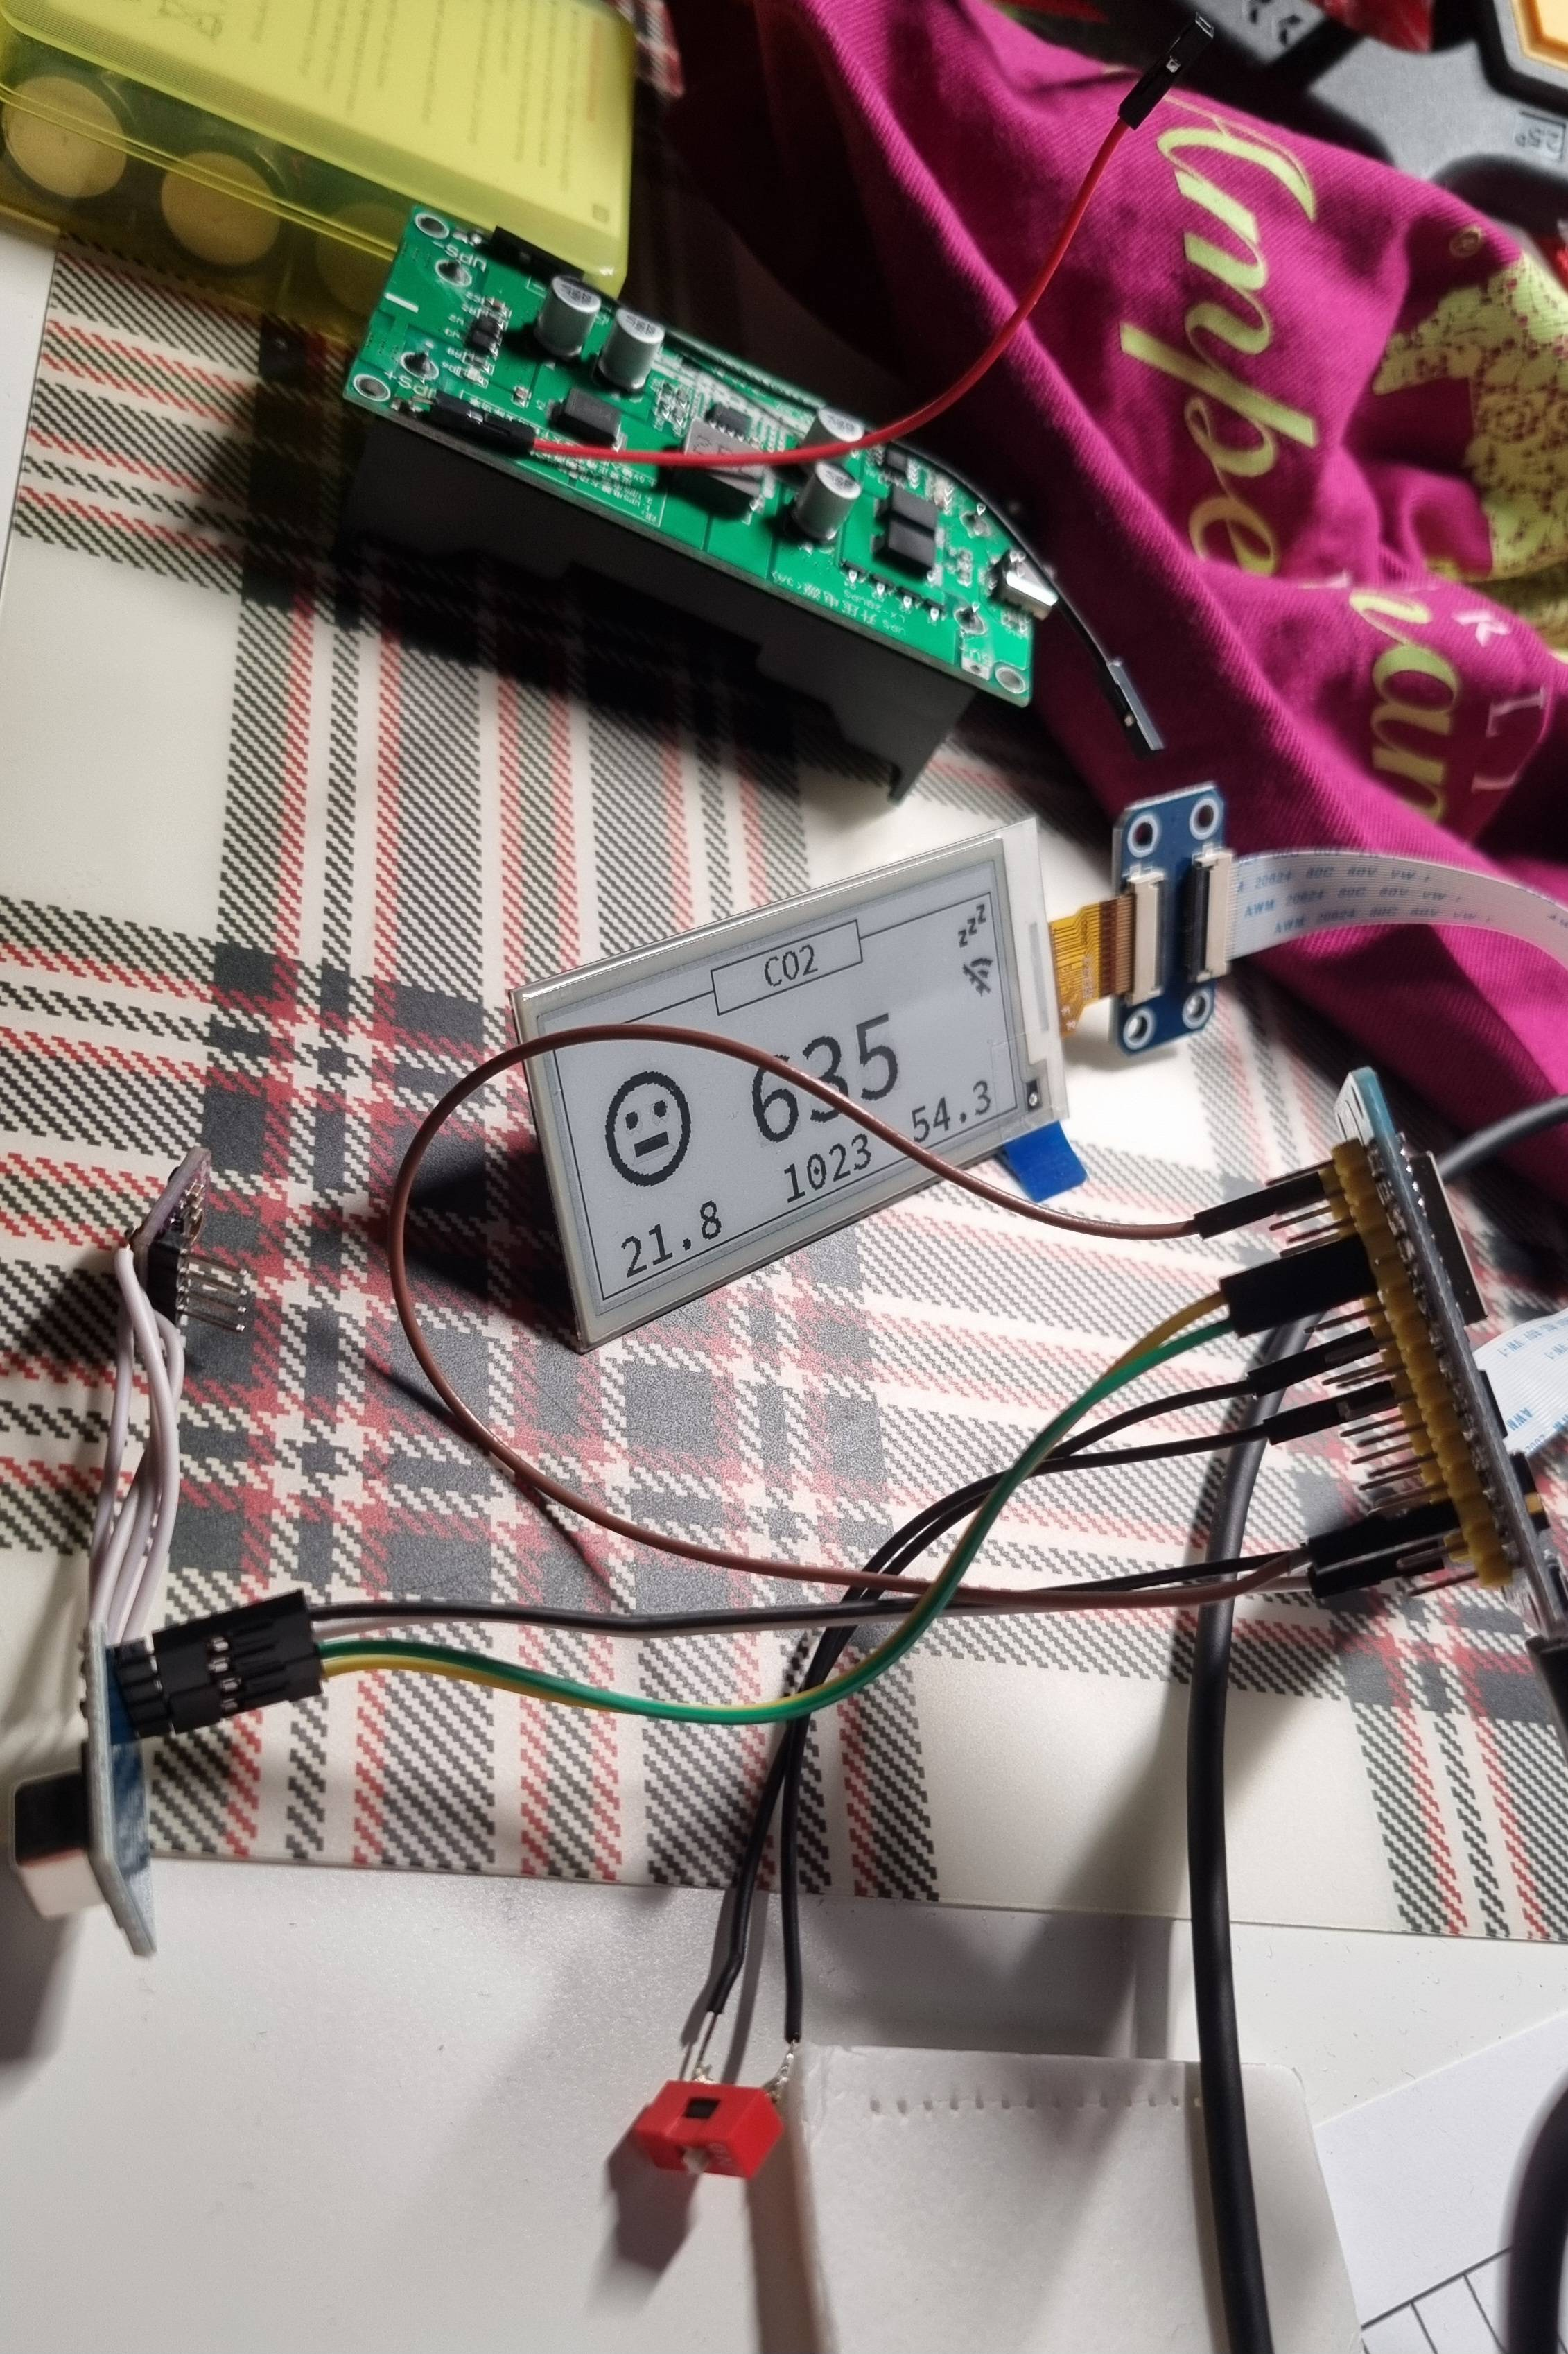
\includegraphics[width=0.9\textheight,angle=90]{bauteile-01.jpg}
\end{frame}

\begin{frame}%[<+->] %%Eine Folie
    \frametitle{Die Bauteile} %%Folientitel
    \begin{description}[<+->][labelwidth=20en]
       \item[Display] Waveshare \SI{2.9}{\inch} ePaper
       \item[Mikrocontroller] ESP8266
       \item[CO2 Sensor] SCD40
       \item[Zusatzsensor] BME280 (\si{\celsius}, \si{\hecto\pascal}, \%RH)
       \item[Akkucontroller] USB-C 18650 Controller von AliExpress
    \end{description}
\end{frame}

\begin{frame}
    \frametitle{Programmierung}
    Foo
\end{frame}

\begin{frame}
    \frametitle{Gehäuse}
    \texttt{boxes.py} to the rescue!\\
    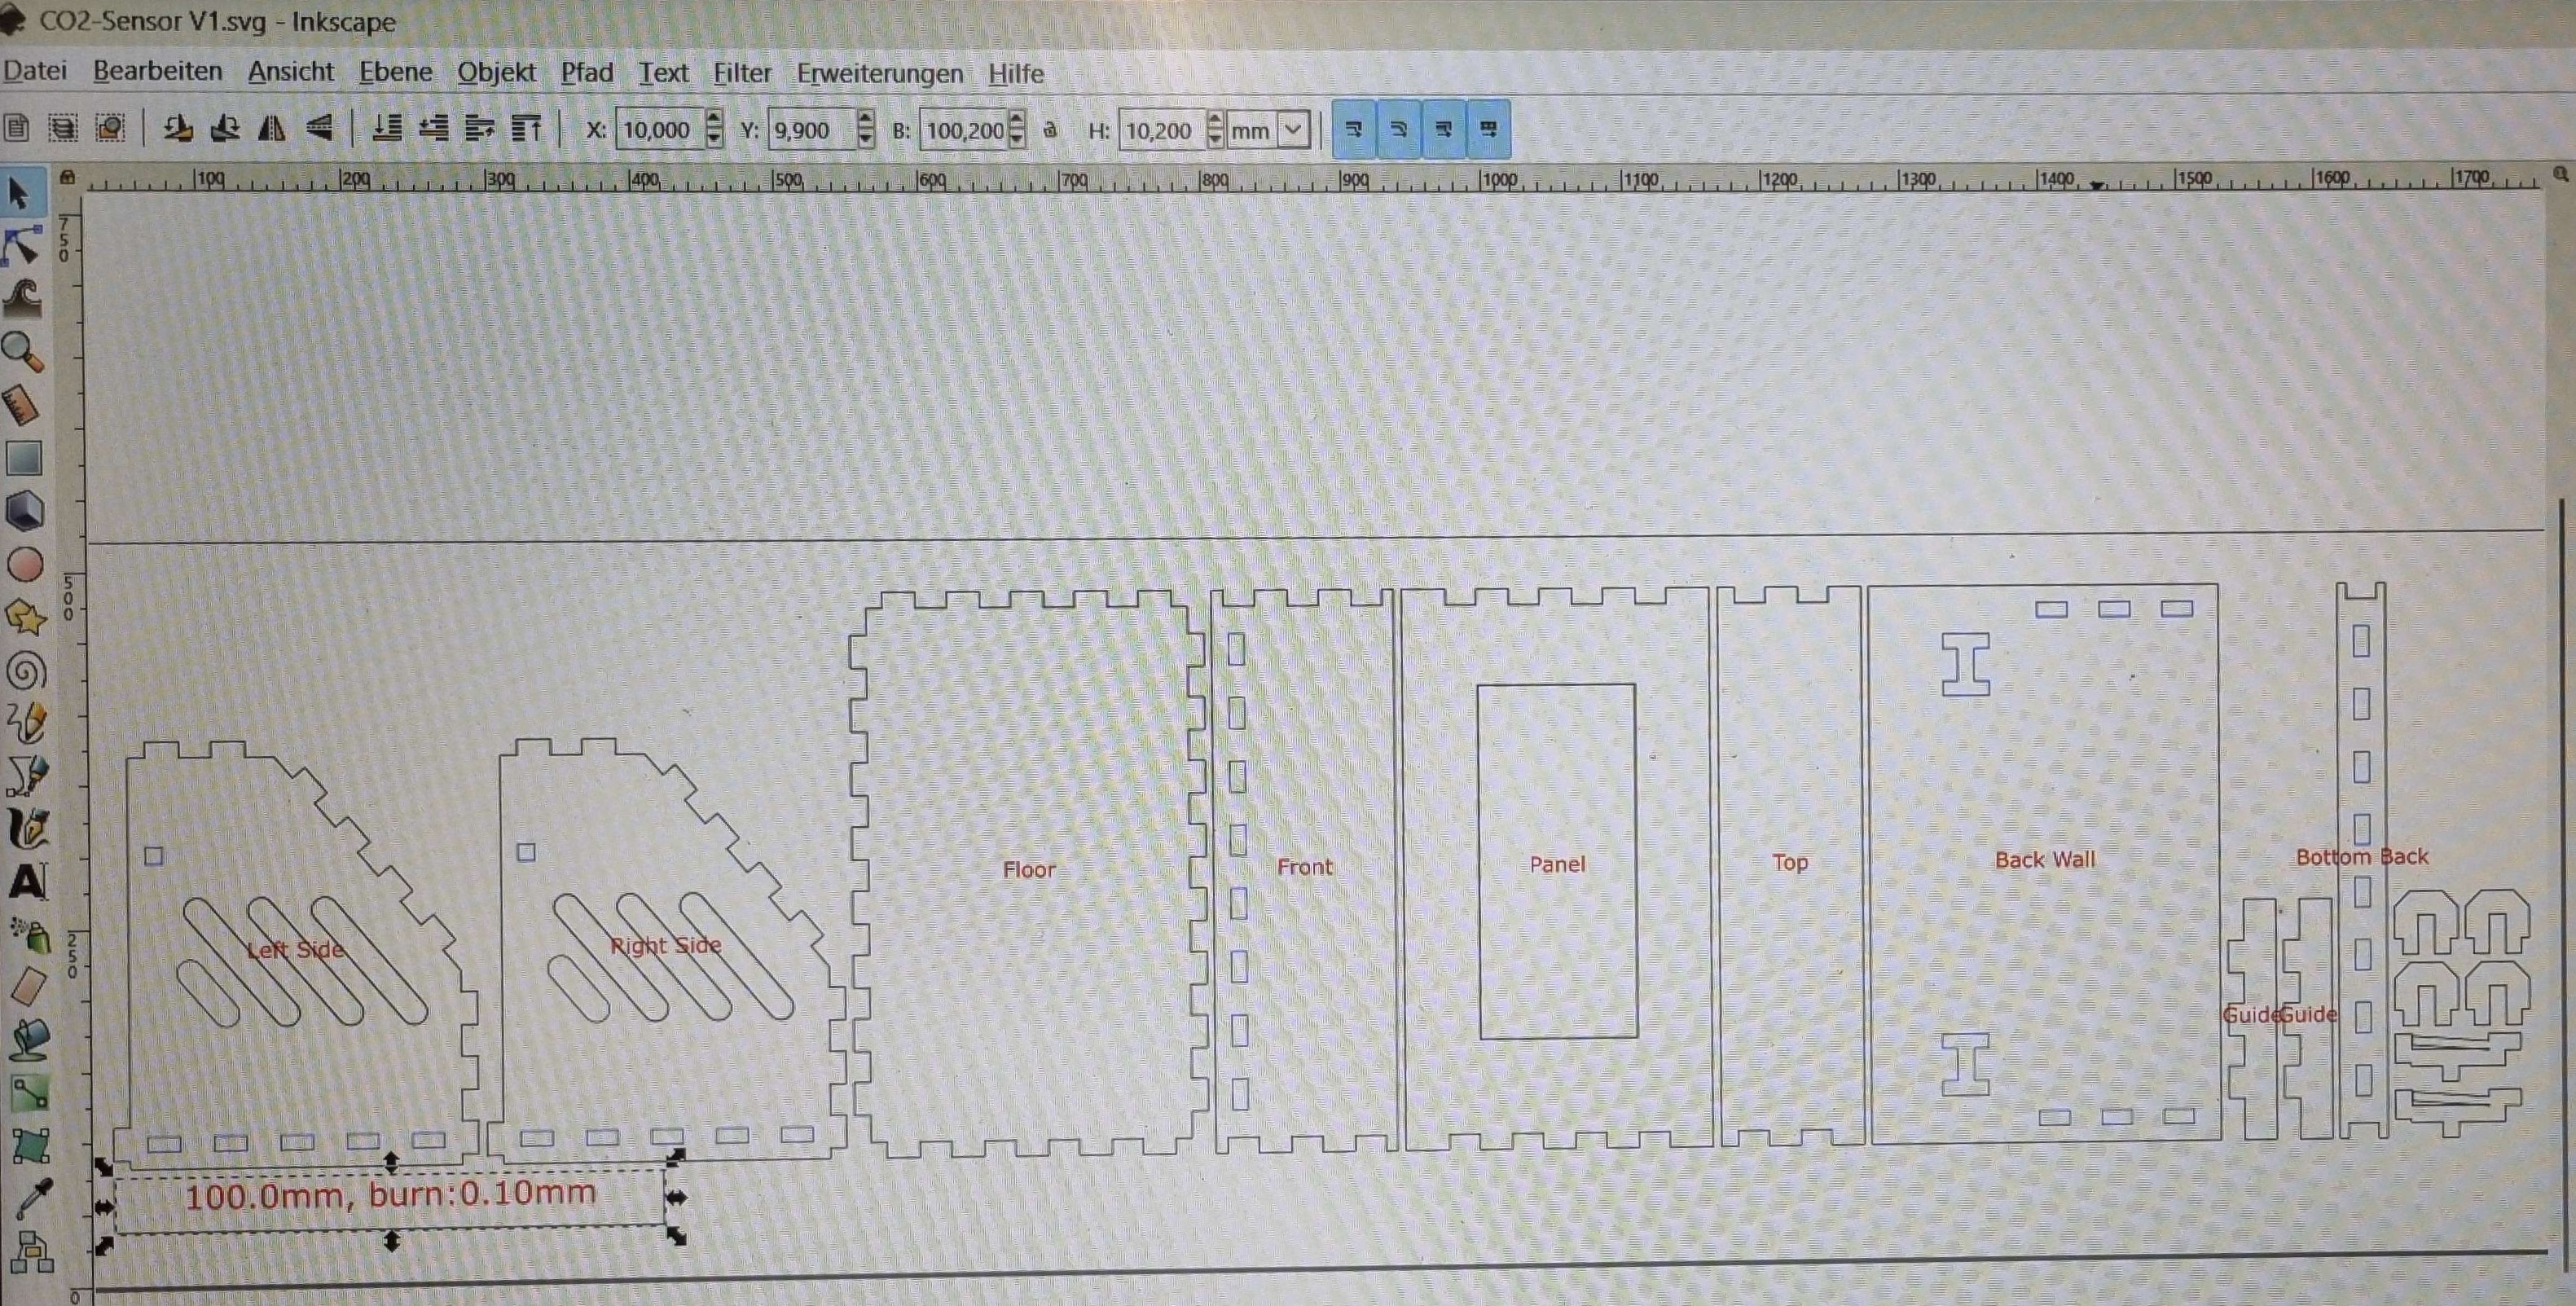
\includegraphics[height=0.8\textheight]{boxes-py-02.jpg}
\end{frame}

\begin{frame}
    \frametitle{Gehäuse}
    \enquote{Laser}\\
    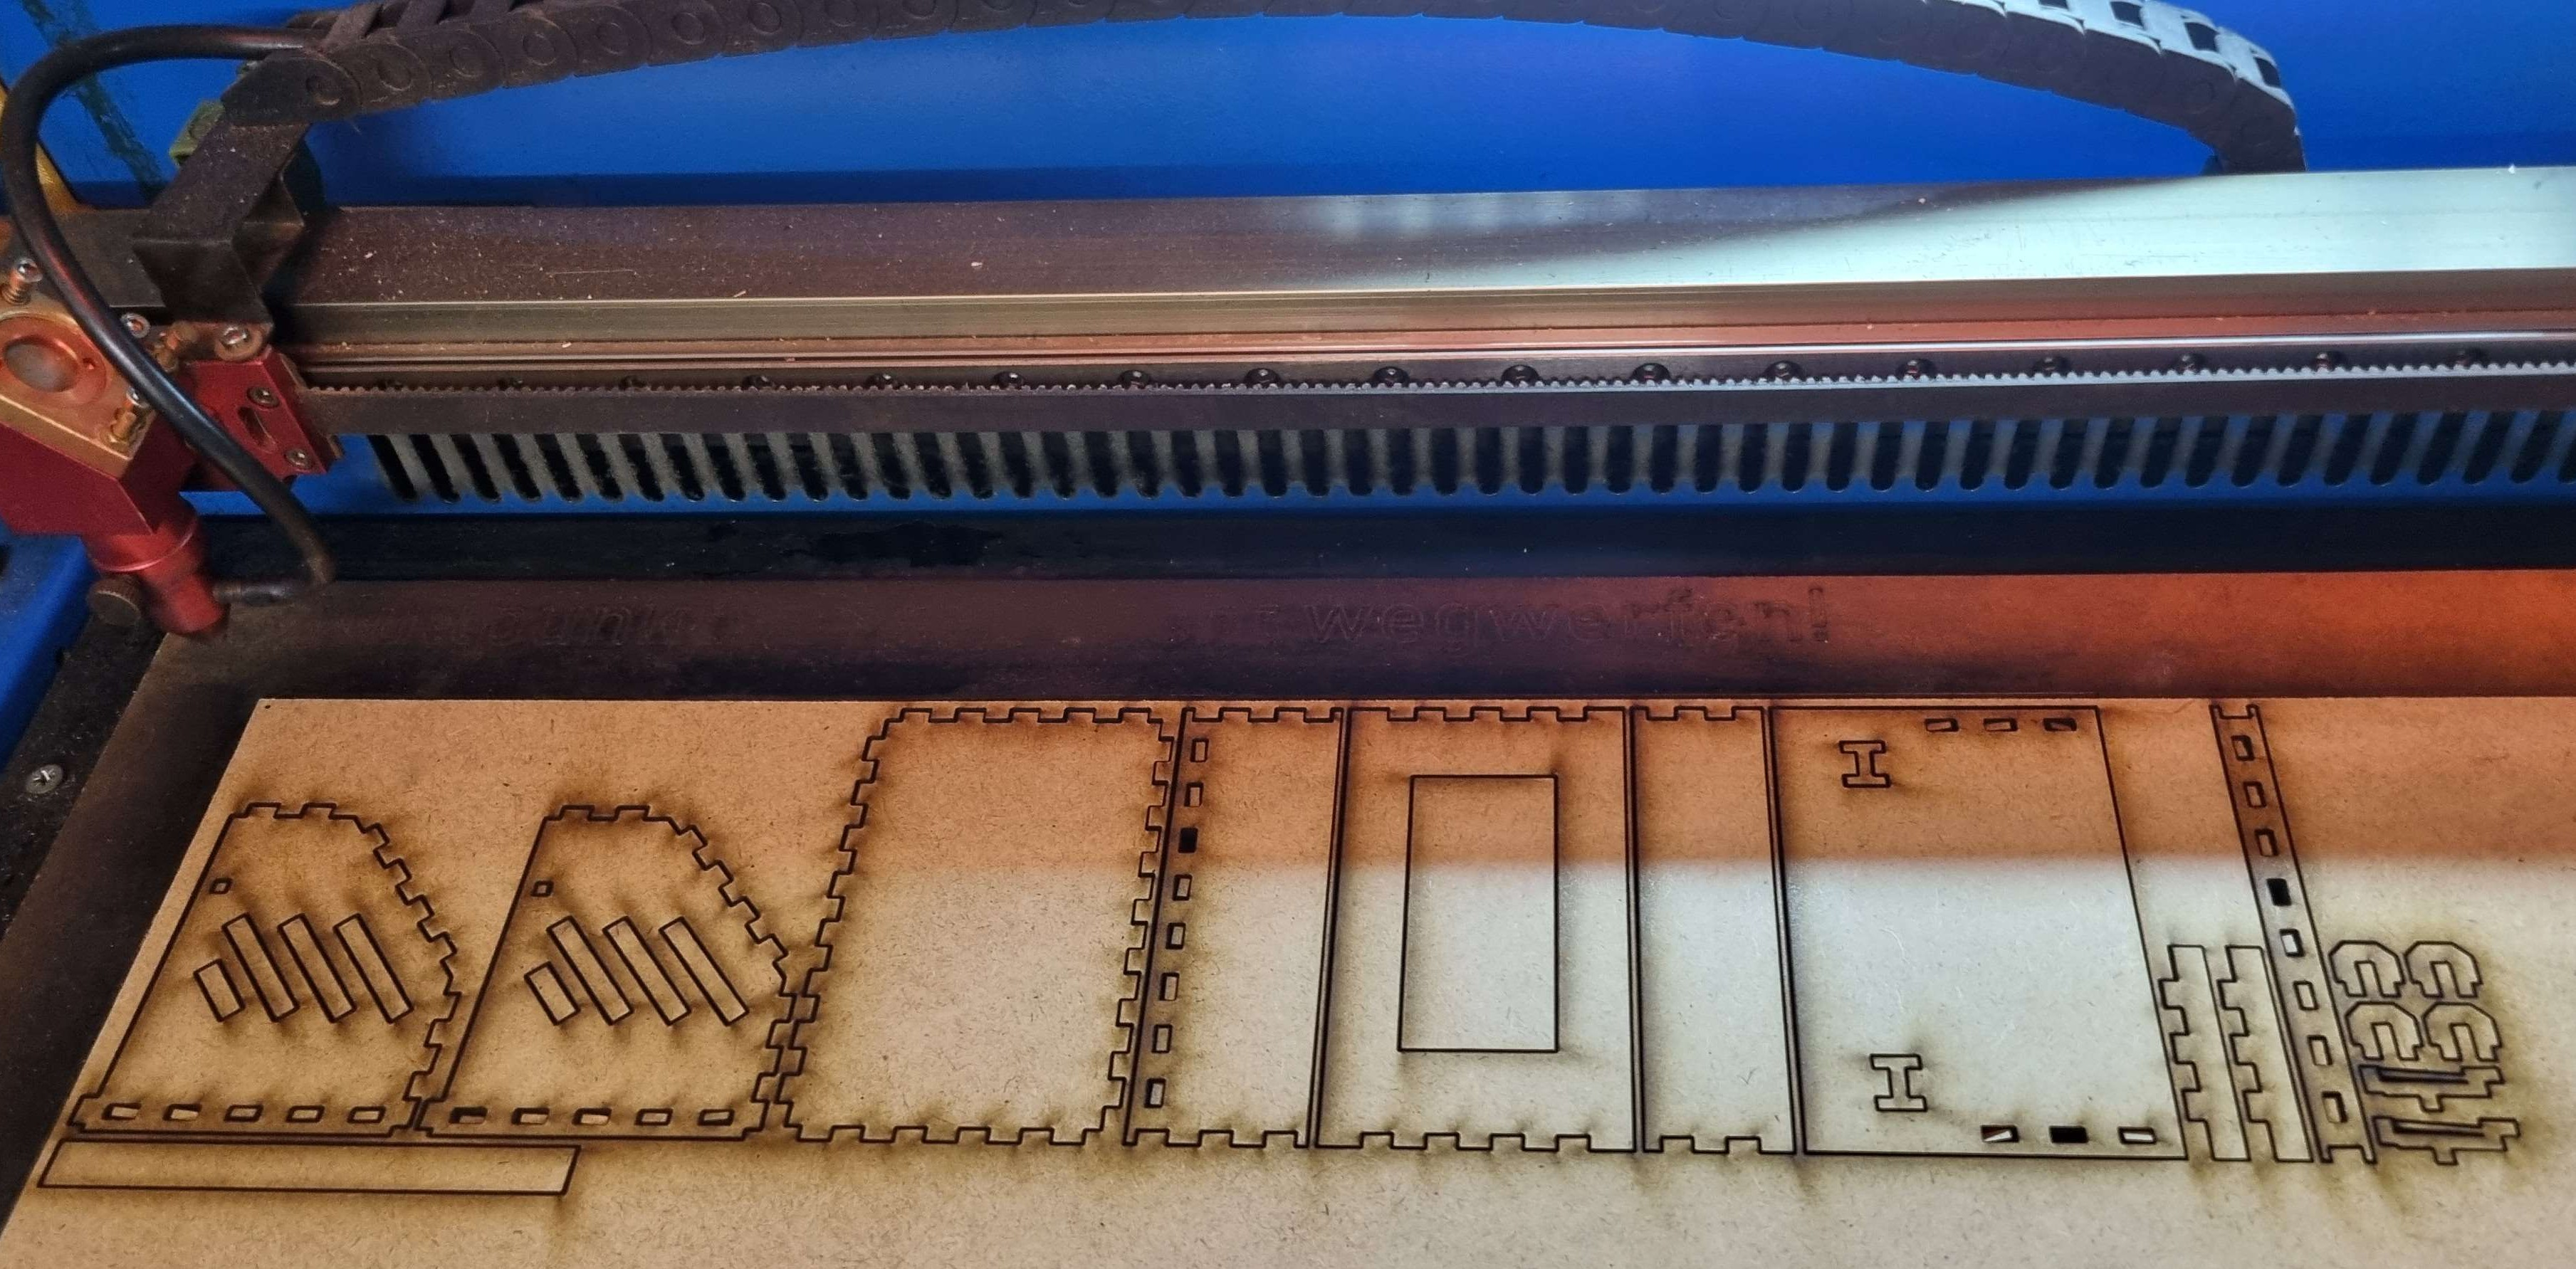
\includegraphics[height=0.8\textheight]{laser-02.jpg}
\end{frame}

\begin{frame}
    \frametitle{Danke für die Aufmerksamkeit!}
    \href{https:\\syralist.de}{syralist.de}
\end{frame}

\end{document}